\documentclass{article}
\usepackage{fancyhdr}
\usepackage{datetime}
\usepackage{parskip}
\usepackage{graphicx}

\pagestyle{fancy}

\fancyhf{}
\fancyfoot[L]{University of Oulu. \today}

\lhead{Waste management system}
\rhead{Page \thepage}

\title{Exercise 1: Design for urban IoT. Waste management system
\author{Andrei Golubev, Hassan Shaheen}
\date{\parbox{\linewidth}{\centering
  \endgraf\bigskip
  University of Oulu
  \endgraf\bigskip\today}}
}

\setlength{\parindent}{0pt}

\begin{document}
\maketitle
\newpage

\section{Abstract}
Household waste has been around throughout the whole humanity lifetime. In current document we
elaborate an idea of (semi-)automated waste management system that aims to simplify everyday human
interaction with wastes. Our idea provides a comprehensive solution to waste management problem.
Multiple tiers of the system are observed to focus both on implementations that are possible today
and also on some that target future technologies.

\section{Concept}

The problem in focus is the waste and the necessity to manage waste utilization and disposal. As a
number of people increases, more waste is produced and requirements for waste management become more
strict and more challenging to satisfy.

Tranditionally, waste management was a manual procedure with different (usually non-optimal) parts.
For example, a person is required to periodically check whether waste bins are full and most likely
remove the content of the bins whether they are empty, half-full or completely full. Not only more
time is spent in this example, there are also additional costs e.g. due to fuel usage (likely a
vehicle is utilized to collect the waste).

Our solution aims to reduce the time and costs spent on waste collection with further improvement in
terms of automation. We believe that the system is beneficial mostly to the city residents rather
than to visitors.

\section{System tiers}

In this section we introduce multiple tiers of the same system so that the reader has better
understanding of possibilities of each tier. Later chapters are explained in terms of the introduced
tiers.

\subsection{Tier 1: Smart waste bins}

This tier is the basic tier of the system. The focus of the system in context of this tier is to
provide "smart" waste bins that are able to measure the waste level inside the bins.

The system consists of a multitude of smart waste bins and a server-side application that aggregates
information from the waste bins (whether they are full or not) and reports the waste bin statuses to
the user of the system (here, a human).

\subsection{Tier 2: Locally automated waste management}

This tier is based on the previous Tier 1. More automation takes place in this system by utilizing
the robots to collect waste individual bins and move them to a centralized waste storage for waste
collection.

The centralized waste storage is a bigger waste collection place that aggregates waste from multiple
households. There can exist one such storage per residential area or even one for the whole
district. The main idea is that such storage is easily accessible by vehicles and requires less time
to collect the waste from. At this level, the management of the centralized waste storage is manual
to a certain degree.

\subsection{Tier 3: Globally automated waste management}

As before, this tier is based on the Tier 2 system. The major difference is a leap from
semi-automated solution to fully automated. The centralized waste storage briefly introduced above
is now fully automated: we rely on autonomous vehicles and extra robotics to take care of waste
aggregation and waste disposal by having similar intelligence, as in the case of smart waste bins,
for the centralized waste storage.

\section{Use cases}

%Describe the audience or users of the application and area or place where the new solution takes
%place. Describe devices involved (e.g. personal devices, public screens and other user interfaces,
%sensors, computing units, etc). Describe users who need the solution and how they benefit using the
%solutions. Use pictures and drawings to show operation of your solution and/or users using it.

Right now, almost 54 percent of the world population lives in urban areas according to the united
nation it will rise to 66 percent by 2050. As the cities are becoming more populated it is putting a
lot of stress on the overall infrastructure. Due to this large-scale urbanization, volume of waste
is increasing; Cities need a smart and efficient waste management system that will replace the
current system where most of the things are done manually.

Our solution is for the city of Oulu and its residents. The system is designed using smart waste
bins that contain fill level sensors and transmit the data to the waste management company.
Utilizing this data, the waste management company will not need any more manual or routine checks,
they can only collect the waste when needed. They can efficiently assign routes to trucks resulting
in less traffic congestion and cutting fuel cost. The city will know how much waste is being
produced so they can evaluate their infrastructure (putting more bins in the area producing more
waste). Residents of Oulu will also benefit from this system, through a mobile app they can find the
nearest empty bin and connect with the company if any assistance is required.

Moreover, remote areas and single households also benefit due to timely waste collection.

\subsection{Tier 1: Smart waste bins}

Our self-aware bins continuously monitor whether they are full or not. The waste level sensor
notifies the central system once a certain level is reached (20\%, 40\%, 80\%, etc.). If the
threshold of, for example, 90\% is reached, the system will put the bin in the collection queue.
This collection queue will help to optimize the route of collection trucks which allows to save on
waste collection costs. At the same time, the level information will help the residents: they can
see by how much a bin is filled and if there is enough space for their waste.

\subsection{Tier 2: Locally automated waste management}

As tier 2 is more automated, we are using robots to collect the waste from residential buildings and
putting them to the centralized storage for that residential area (and nearby areas), from where it
can be collected by trucks and taken into waste processing plants. Other parts of the system will
work the same way: a bin will notify the system and instead of putting it into the collection queue
of the trucks, a robot will be assigned to that bin. The bins will have RFID tags through which the
robot reads the information about an individual bin. The information includes geo data so that it is
easy to determine where to put the bin after it is emptied, bin type (biowaste, plastic, etc.) and
other.

Thus, such a robot can move the bin to the waste storage and return it back to the right place.
These bins are designed in the way that makes it easier for the robot to attach/pick them. This
process will eradicate the need for waste trucks in residential areas reducing noise and air
pollution and cutting costs even more. We propose to use some simple computer vision-based
technology for the robot to understand how to attach to the bin (e.g. black and white markers on the
bin surface).

\subsection{Tier 3: Globally automated waste management}

Tier 3 will be a fully automated waste management system where human interaction is not required or
is extremely limited. The idea is the following: bins notify the system about their level, system
assigns the robot to collect the bin, the robot gets the bin and takes it to the assigned storage
and then puts the bin back to the residential building. Instead of collection trucks operated by
humans, autonomous vehicles will collect the waste from the centralized storage and take it to the
waste processing plant. The fully automated system will be more efficient, more environment friendly
and less costly for the city.

\section{Methodology}

% Propose a technical solution for implementation of your design. How do the participating devices
% communicate? What are sensors and actuators your design uses? What kind of data is collected, and
% how it needs to be processed? Where does the computation happen (in local devices, cloud, somewhere
% else)? Use graphs and images.

In this section we explore possible technical implementation for each system tier.

\subsection{Tier 1: Smart waste bins}

\begin{figure}[ht!]
\centering
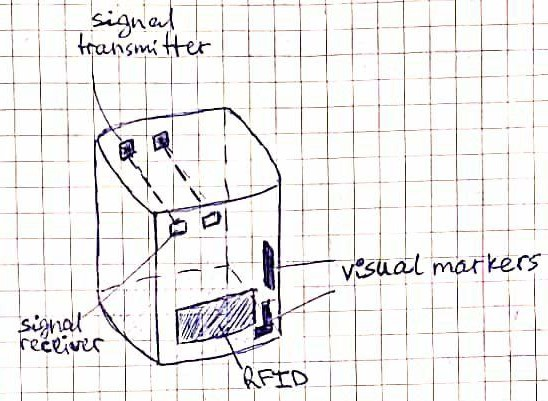
\includegraphics[width=90mm]{./waste_bin.jpg}
\caption{Smart waste bin components}
\end{figure}

We propose to use a simple waste level control system for waste bins. Each bin has the following
components:

- There is an attached IoT device (e.g. Arduino or other microcontroller) and the device has a
wireless network connection (WiFi, Internet, etc.)

- The waste bin is able to indentify whether it is full or close to being full. This is achieved by
a sensor (e.g. infrared) that monitors the number of waste inside the bin and reports the
measurements to the IoT device for processing

- Laser transmitter and receiver are used to understand the waste level: transmitter emits signal
that is caught by the receiver, once the signal stops arriving, it means that something (waste)
prevents the laser from propagating. Utilizing multiple horizontal transmitter-receivers (TRs)
allows to control whether the waste is uniformly placed inside the bin. Several horizontal levels of
TRs provide the capability to control waste level in a percentage manner (20\%, 40\%, etc.).

- RFID marker  is added on the outside surface of the bin to address "future" functionality
available in Tier 2 system.

- Visual markers are installed across the outer faces of the bin to enable automated vision-based
understanding of the bin shape and structure.

Figure 1 shows a scheme of the essential smart bin components.

\subsection{Tier 2: Locally automated waste management}

The main technology introduced in this tier is robotics. As this tier is targeting the future use
case, we cannot fully elaborate the technical specification for the robot. However, since there
exist many industrial and household robotics solutions, we can describe requirements:

- The robot must have movement components to be able to move along surfaces in all directions. The
movement mechanism must be rather robust as different road conditions exist e.g. asphalt, gravel,
ice.

- Computer vision system must be present so that the robot can detect the specific bin face on which
RFID tag as well as handles are located. The system does not have to be extraordinary, some simple
industrial-inspired solution may apply perfectly. Nonetheless, the implementation must be robust due
to different challenges present in the field (e.g. varying lighting conditions).

- RFID reader must be installed on the robot to read the unique bin data on the bin.

- The robot must be able to hold and move the waste bin. We suggest to install wheels on the bin
itself so that the weight of the waste does not affect the required force much. Additionally,
special handles may be added to the bin so that it is easier for the robot to attach to the bin.

TODO: anything else here? - about centralized waste storage

\subsection{Tier 3: Globally automated waste management}

\begin{figure}[ht!]
\centering
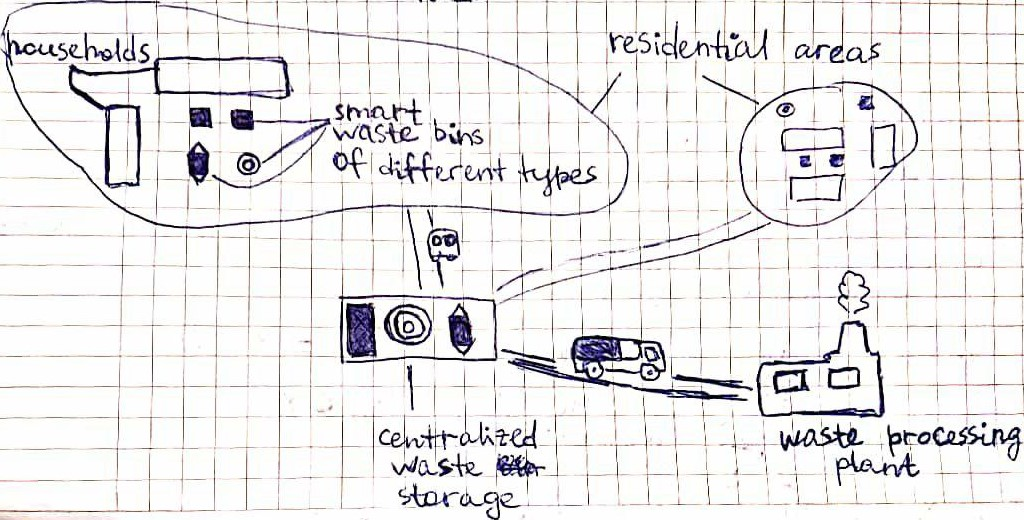
\includegraphics[width=110mm]{./high_level_scheme.jpg}
\caption{System overview}
\end{figure}

Figure 2 shows the overview of the whole system with the main components.

\subsection{Communication}


\section{Technical challenges}
TODO: challenges with bin fulfillment check (imperfections in IR, etc)

\section{Outcomes and conclusion}


\end{document}
